\documentclass{../../vmdm}

\begin{document}
\boxedpoints

\VMDMTitre{septembre 2022 (4ème)}
\vspace{0.2cm}
\VMDMRegles{}
\vspace{0.2cm}

\qformat{Exercice \thequestion \dotfill (\totalpoints~points)}
\begin{questions}
    \question \leavevmode%
    \begin{mdframed}[leftmargin=2cm, rightmargin=2cm]
        \underline{Programme de calcul}
        \begin{itemize}
            \item Choisir un nombre entier impair
            \item Le multiplier par 5
            \item Enlever 7 au résultat précédent
            \item Diviser par 2 le résultat précédent
        \end{itemize}
    \end{mdframed}
    \begin{parts}
        \part[1] Quel résultat obtient-on si on choisit le nombre 11 ? \rep{24}
        \part[1] Quel résultat obtient-on si on choisit le nombre 3 ? \rep{4}
        \part[2] Que dire du résultat si on choisit un nombre pair au départ ?
    \end{parts}

    \question[12] \leavevmode%
    \begin{mdframed}[leftmargin=5cm, rightmargin=5cm]
        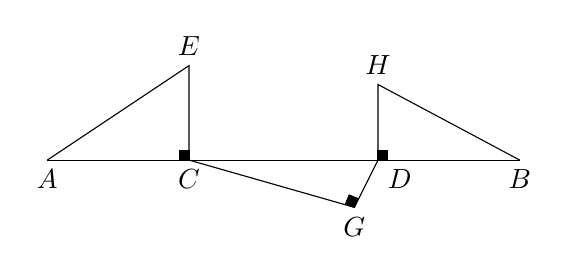
\begin{tikzpicture}[scale=0.6]
            \draw (0,0) node[below] {$A$} -- (10,0) node[below] {$B$};
            \draw (3,0) node[below] {$C$} -- (3,2) node[above] {$E$} -- (0,0);
            \draw (3,0) -- (6.5,-1) node[below] {$G$} -- (7,0) node[below right] {$D$};
            \draw (7,0) -- (7,1.6) node[above] {$H$} -- (10,0);
            \draw[fill=black] (3,0) rectangle (2.8,0.2);
            \draw[fill=black,rotate around={68:(6.5,-1)}] (6.5,-1) rectangle (6.7,-0.8);
            \draw[fill=black] (7,0) rectangle (7.2,0.2);
        \end{tikzpicture}
    \end{mdframed}

    Sachant que $AE = \qty{6}{cm}$, $CE = \qty{3.38}{cm}$, $CG = \qty{6}{cm}$, $GD=\qty{4.34}{cm}$, $DH = \qty{2.2}{cm}$ et $BH = \qty{7}{cm}$, déterminer la distance $AB$. \rep{\qty{19}{cm}}
 
    \question 
    \begin{parts}
        \part[1] Calculer $87 \div 99$
        \part[1] Calculer $12 \div 99$
        \part[1] Que remarque-t-on ?
        \part[1] Donner une fraction égale à $12{,}47474747...$
    \end{parts}
\end{questions}


\vfill

\begin{center}
\gradetable[h][questions]
\end{center}

\end{document}